\documentclass[conference]{IEEEtran}

% *** GRAPHICS RELATED PACKAGES ***
%
\ifCLASSINFOpdf
   \usepackage[pdftex]{graphicx}
  % declare the path(s) where your graphic files are
  % \graphicspath{{../pdf/}{../jpeg/}}
  % and their extensions so you won't have to specify these with
  % every instance of \includegraphics
  % \DeclareGraphicsExtensions{.pdf,.jpeg,.png}
\else
  % or other class option (dvipsone, dvipdf, if not using dvips). graphicx
  % will default to the driver specified in the system graphics.cfg if no
  % driver is specified.
  % \usepackage[dvips]{graphicx}
  % declare the path(s) where your graphic files are
  % \graphicspath{{../eps/}}
  % and their extensions so you won't have to specify these with
  % every instance of \includegraphics
  % \DeclareGraphicsExtensions{.eps}
\fi

% *** MATH PACKAGES ***
%
\usepackage{amsmath}
\usepackage{mathtools}
\DeclarePairedDelimiter\floor{\lfloor}{\rfloor}

% *** SUBFIGURE PACKAGES ***
\ifCLASSOPTIONcompsoc
 \usepackage[caption=false,font=normalsize,labelfont=sf,textfont=sf]{subfig}
\else
 \usepackage[caption=false,font=footnotesize]{subfig}
\fi


% *** PDF, URL AND HYPERLINK PACKAGES ***
%
\usepackage{url}


\usepackage[brazilian]{babel}
\usepackage[utf8]{inputenc}
%\usepackage[T1]{fontenc}
\usepackage{fancyhdr}


% correct bad hyphenation here
%\hyphenation{op-tical net-works semi-conduc-tor}


\pagestyle{fancy}
%\fancyhf{}
\chead{VII Workshop de P\'{o}s-Gradua\c{c}\~{a}o - Engenharia de Computa\c{c}\~{a}o - WPGEC 2018}
\renewcommand{\headrulewidth}{2pt}

\pagenumbering{gobble}

\begin{document}

%
% paper title
% Titles are generally capitalized except for words such as a, an, and, as,
% at, but, by, for, in, nor, of, on, or, the, to and up, which are usually
% not capitalized unless they are the first or last word of the title.
% Linebreaks \\ can be used within to get better formatting as desired.
% Do not put math or special symbols in the title.
\title{Paper title - English \\ T\'{i}tulo do artigo - somente para documento escrito em Portugu\^{e}s}



% conference papers do not typically use \thanks and this command
% is locked out in conference mode. If really needed, such as for
% the acknowledgment of grants, issue a \IEEEoverridecommandlockouts
% after \documentclass

% for over three affiliations, or if they all won't fit within the width
% of the page, use this alternative format:
% 
\author{\IEEEauthorblockN{BRAGA, Samira J.\IEEEauthorrefmark{1};
GOMI, Edson S.\IEEEauthorrefmark{1}}
\IEEEauthorblockA{\IEEEauthorrefmark{1}Escola Politécnica da Universidade de São Paulo}}


% make the title area
\maketitle

\thispagestyle{fancy}

% As a general rule, do not put math, special symbols or citations
% in the abstract
\renewcommand{\abstractname}{Abstract}
\begin{abstract}
Abstract here.
\end{abstract}

\renewcommand\IEEEkeywordsname{Keywords}
\begin{IEEEkeywords}
\label{Keywords}
word 1; word 2.
\end{IEEEkeywords}

\renewcommand{\abstractname}{Resumo}
\begin{abstract}
\label{Resumo}
\'E necess\'aria a inser\c{c}\~{a}o do resumo para artigo escrito em Portugu\^{e}s.
\end{abstract}

\renewcommand\IEEEkeywordsname{Palavras-chave}
\begin{IEEEkeywords}
\label{Palavras-chave}
palavra 1; palavra 2.
\end{IEEEkeywords}

\renewcommand\IEEEkeywordsname{Classifica\c{c}\~{a}o}
\begin{IEEEkeywords}
	\label{classificacao}
	Mestrado
\end{IEEEkeywords}

\renewcommand\IEEEkeywordsname{Categoria}
\begin{IEEEkeywords}
	\label{Categoria}
	Iniciante 
\end{IEEEkeywords}

\IEEEpeerreviewmaketitle


\section{Introdução}

%avaliação da espessura numa area mais extensa (nao só no circulo) melhora a capacidade de diagnostico?

\section{Diagnóstico de glaucoma}

%o que e glaucoma (tese marcelo)
%como e feito o diagnostico
%oct no diagnostico

Glaucoma é uma neuropatia óptica crônica multifatorial e de lenta progressão que causa perda de campo visual periférico e é a segunda maior causa de cegueira no mundo, estima-se que atingirá 79,6 milhões de pessoas até 2020 \cite{Quigley2006}. Essa doença caracteriza-se pela perda da camada de fibras nervosas no olho, o que pode causar cegueira se não for tratado corretamente \cite{Quigley2011}. O dano na camada de fibras nervosas se dá antes de alteração no campo visual do paciente, por isso o diagnóstico precoce é um fator importante para evitar a perda da visão \cite{Malik2012}.

O glaucoma é diagnosticado por meio do exame perimetria computadorizada (SAP), que é um exame funcional, e pela tomografia de coerência óptica (OCT), que é um exame estrutural. Os exames funcionais avaliam o campo visual do paciente em busca de reduções na visão. Os exames estruturais avaliam a camada de fibras nervosas para identificar alterações na espessura. Não é simples identificar a existência do glaucoma antes que haja dano ao campo visual \cite{Populacoes2009}.

O OCT é empregado para identificar alterações na espessura da camada de fibras nervosas. No exame, utiliza-se o princípio da interferometria luminosa para medir as espessuras das estruturas intraoculares. Ao realizar uma varredura, o equipamento emite feixes de laser infravermelho e mede o tempo que a luz leva para ser refletida. A cada estrutura atravessada, uma parte dessa luz é refletida de volta, é feito então o cálculo da espessura da estrutura com base em um feixe de luz de referência e o quanto de luz foi refletido de volta \cite{huang1991}. 

Durante o exame com um equipamento de alta definição, são realizadas $200$ varreduras lineares verticais e $200$ horizontais em uma área de 6mm centralizado no disco óptico, após isso é gerada uma saída como na figura \ref{fig:oct}. O primeiro gráfico no topo representa o mapa de espessuras de toda a área analisada, as áreas sem azul indicam espessuras próximas a $0$ e áreas amarelas e vermelhas indicam espessuras entre $175$ e $350$ mícrons. O disco central em cinza representa a fóvea, ponto cego do olho de onde sai o nervo óptico. Abaixo do mapa de espessuras está a o mapa de desvio, mostra as áreas onde a espessura está diferente da população normal, de acordo com um banco de dados normativo do software do equipamento. Também nesse gráfico está representada a linha círcular de onde são retirados os pontos para a representação da espessura nos gráficos na parte de baixo da saída. Esses gráficos mostram a espessura ao longo da circunferência, com centro no nervo óptico. A partir dos ponto dessa circunferência, são gerados os gráficos de quadrantes e horas de relógio, que representam as espessuras médias em cada região.

É possível utilizar classificadores de aprendizagem de máquina para fazer o diagnóstico de glaucoma com base nos exames de OCT e SAP. Um classificador de rede neural profunda foi utilizado com dados de exame de campo visual para detectar estágios iniciais de glaucoma \cite{Asaoka2016}. Dados de OCT e SAP em conjunto também foram utilizados para treinar diversos tipos de classificadores \cite{bowd2008,Populacoes2009}. %Não foi encontrado na literatura o uso dos valores de espessura de toda a área medida pelo OCT como entradas para um classificador. 

% classificadores com parametros de oct (horas de relogio) e sap
%pegar imagem do oct para utilizar toda a area de espessura do nervo para usar no diagnostico

\begin{figure}[!tp]
  \centering
  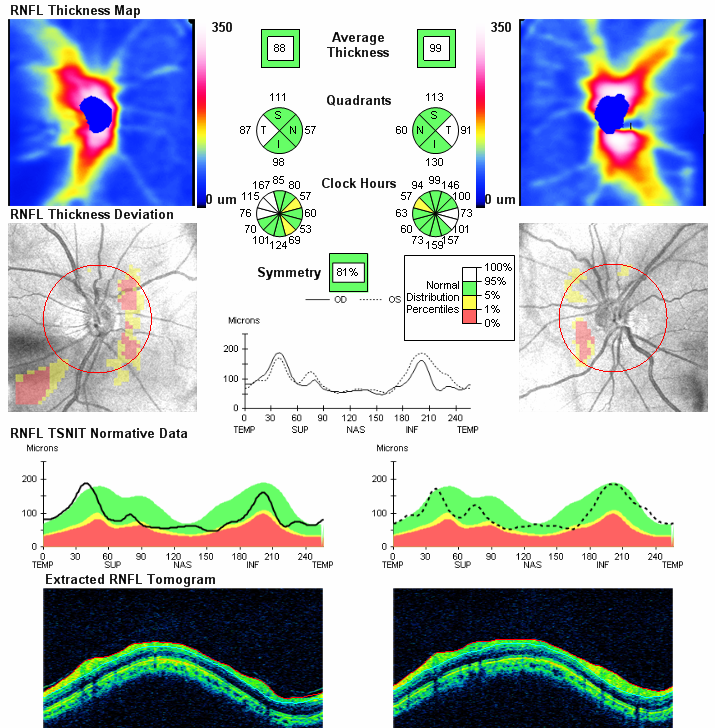
\includegraphics[width=2.5in]{img/oct.png}
  \caption{Saída de um exame de OCT.}
  \label{fig:oct}
\end{figure}

\section{Redes neurais convolucionais}

\begin{figure*}[!t]
  \centering
  \subfloat[Imagem de entrada da rede]{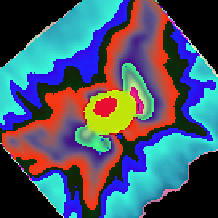
\includegraphics[width=1in]{img/conv/data}%
  \label{fig:data}}
  \hfil
  \subfloat[Imagem de saída da primeira camada convolucional]{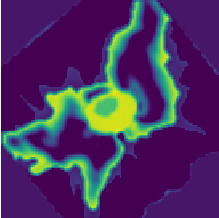
\includegraphics[width=1in]{img/conv/conv1_1}%
  \label{fig:conv1}}
  \hfil
  \subfloat[Imagem de saída da segunda camada convolucional]{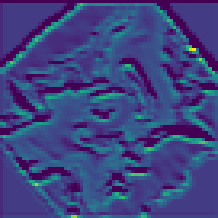
\includegraphics[width=1in]{img/conv/conv2_1}%
  \label{fig:conv2}}
  \hfil
  \subfloat[Imagem de saída da terceira camada convolucional]{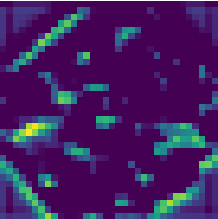
\includegraphics[width=1in]{img/conv/conv3_1}%
  \label{fig:conv3}}
  \hfil
  \subfloat[Imagem de saída da quarta camada convolucional]{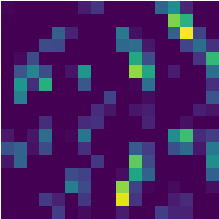
\includegraphics[width=1in]{img/conv/conv4_1}%
  \label{fig:conv4}}
  \hfil
  \subfloat[Imagem de saída da quinta camada convolucional]{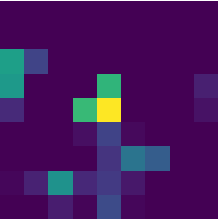
\includegraphics[width=1in]{img/conv/conv5_1}%
  \label{fig:conv5}}
  \caption{Exemplos de saídas de cada camada convolucional ao longo da rede.}
  \label{fig:imagens_rede}
\end{figure*}

%o que sao redes convolucionais
%explicar cada tipo de camada
%imagens das saidas em cada convolucional

Redes neurais profundas estão sendo amplamente utilizadas em diversos domínios para classificação e detecção de objetos, principalmente em visão computacional e reconhecimento e processamento de linguagem natural. Essas redes consistem em várias camadas conectadas que aprendem a reconhecer padrões nos dados apresentados, sejam eles imagens ou sons. O principal tipo de rede utilizado é a rede neural convolucional (RNC). As RNCs mostraram ser excelentes ferramentas no processamento de imagens, inclusive na área médica, sendo utilizadas para classificação, detecção de objetos e segmentação \cite{greenspan2016}. Esse sucesso deve-se principalmente à utilização de grandes quantidades de exemplos de treinamento, que permitem que a rede aprenda a reconhecer características a partir dos dados brutos das imagens. %raw data?

As RNCs são compostas de várias conectadas, os principais tipos de camadas são as convolucionais, pooling e as camadas totalmente conectadas. As camadas convolucionais servem como filtros para identificar as características das imagens, como curvas, bordas e cores. As saídas das camadas convolucionais são mapas de características identificadas na imagem de entrada. A convolução é feita utilizando uma máscara (ou kernel) que desliza por todos os pixels da imagem múltiplicando os valores do pixel pelos valores da máscara. Essa múltiplicação é feita em toda a imagem com diferentes kernels, gerando assim as saídas dos diferentes filtros.

Após a identificação dessas características, a camada de pooling agrupa as características similares e reduz a resolução da imagem. Também utilizando uma máscara, a operação de pooling irá calcular o valor máximo em cada região da imagem, agrupando características similares em um mesmo pixel. Na figura \ref{fig:imagens_rede} é possível acompanhar o agrupamento de características e a redução da resolução da imagem ao longo de 5 camadas convolucionais e pooling.



\begin{figure}[!tp]
  \centering
  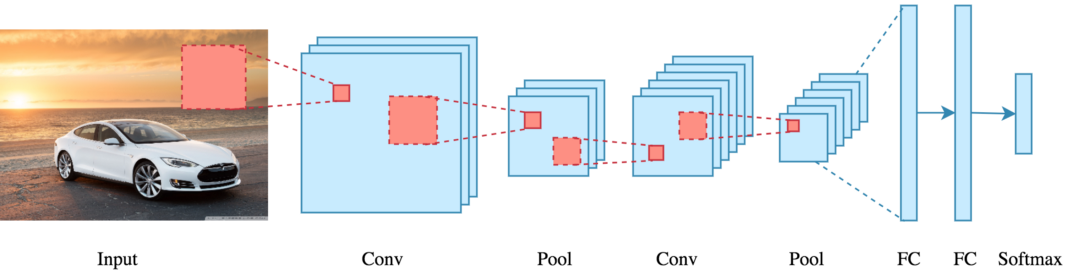
\includegraphics[width=2.5in]{img/convolucao.png}
  \caption{Esquema de camadas de uma rede neural convolucional.}
  \label{fig:convolucao}
\end{figure}


  \subsection{Transfer Learning}

  %como e feito transfer learning

  \subsection{Redes pré-treinadas}

  %explicar vgg

\section{Experimentos e resultados}

%setup do servidor, quais gpus
%utilizando caffe
%qual o objetivo dos experimentos, como foi avaliado

% Os experimentos foram conduzidos em um servidor com Ubuntu 16.04 com duas GPUs NVidia Quadro K5200 com 8GB de memória cada, 24 CPUs Intel Xeon e 128GB de memória RAM. O framework de deep learning utilizado em todos os experimentos foi o Caffe, fornecido pela universidade de Berkeley \cite{jia2014caffe}.

% O objetivo dos experimentos, com e sem transfer learning, é a classificação binária de olhos normais ou com glaucoma em imagens de OCT. A performance das redes foram avaliadas utilizando um conjunto menor de imagens não vistas para classificação e cálculo das métricas de avaliação. O mesmo conjunto de imagens é utilizado em todos os experimentos. O dataset, pré-processamento e resultados são descritos em detalhes nas próximas seções.

  \subsection{Dataset}

  %aumento do dataset, rotações aleatorias entre 0 e 360
  %divisao treino e validação

  O dataset original foi obtido com o departamento de oftalmologia da Unicamp. O dataset consiste de imagens de OCT com tamanho 136x136 de 56 olhos com glaucoma e 66 olhos normais, totalizando 122 pacientes. Os gráficos de espessura de fibras nervosas foram obtidos através da extração das imagens do PDF do exame. Foram selecionados para o experimento somente os olhos de pacientes que foram manualmente classificados por especialistas.

  Para a separação do dataset em treino e validação, foram selecionados 20\% de olhos normais e 20\% de olhos com glaucoma para validação, e o restante para treino, totalizando 98 imagens de treino e 24 para validação. As imagens selecionadas para teste não estão presentes no dataset de treino, para que o algoritmo possa classificar imagens ainda não vistas.

  Para evitar overfitting, foi empregada uma técnica para aumentar o número de exemplos a partir das imagens no dataset de treino. Cada imagem foi rotacionada 100 vezes em ângulos aleatórios entre 0 e 360 graus, gerando assim um dataset de treino com 9800 imagens. As imagens de validação não foram rotacionadas.

  \subsection{Pré-processamento}

  % subtração da media
  % areas pretas para zero absoluto

  %formula do calculo do pixel medio
  
  %gerar saida da imagem media, calcular desvio padrao, gerar imagens com media+desvio padrao e media-desvio padrao
  
  Para utilização do transfer learning, foi necessário fazer a subtração do pixel médio em todas as imagens do dataset de treino. O valor (médio de cada pixel da imagem) é calculado sobre todas as imagens do dataset de treino. Essa imagem média é então subtraída de cada imagem do dataset. Dessa forma, todos os pixels de entrada estão na mesma ordem de grandeza, evitando que os gradientes desapareçam ou explodam.

  Onde houveram falhas na aquisição da imagem, gerando áreas escuras, pixels com valores RGB próximos ao preto foram substituídos pelo valor de preto absoluto RGB (0, 0, 0) para que não tenham influência sobre a decisão do classificador.

  \subsection{Resultados com transfer learning}

  %estrategia de learning rate
  %iterações e tempo de processamento
  %grafico da acuracia


  Neste experimento, utilizamos a mesma arquitetura da rede VGG16, alterando a saída da última camada totalmente conectada para duas saídas, correspondente às duas classes a serem classificadas: normal e glaucoma. A camada de entrada da rede também foi alterada para a resolução das imagens do nosso dataset. As imagens do dataset Imagenet com que a rede foi treinada tinham a resolução de 224x224 pixels, enquanto que as imagens de OCT têm resolução de 136x136 pixels.
  
  Os pesos pré-treinados foram carregados para inicialização apenas das camadas convolucionais. As três últimas camadas totalmente conectadas foram iniciadas com valores aleatórios devido à diferença de resolução entre as imagens do dataset Imagenet e as imagens de OCT classificadas nesse experimento. Essa diferença gera quantidades de parâmetros diferentes na saída da última camada convolucional. Sendo assim, as camadas totalmente conectadas foram inicializadas com valores aleatórios de uma distribuição normal com desvio padrão $0.01$.

  O treinamento foi realizado em todas as camadas da rede, utilizando o gradiente descendente estocástico por $5000$ iterações, com mini batches de $15$ imagens. Os parâmetros de momentum e weight decay foram definidos como $0.9$ e $0.0005$, respectivamente. A taxa de aprendizagem inicial foi de $0.001$. A cada $1000$ iterações a taxa de aprendizagem foi diminuída utilizando a equação \ref{eq:learning_rate}.

  \begin{equation}
    base\_lr * \gamma^{\floor*{\frac{iter}{step}}}
    \label{eq:learning_rate}
  \end{equation}

  Onde $base\_lr$ é a taxa de aprendizagem inicial, $\gamma$ é um parâmetro do Caffe definido com o valor $0.1$, $iter$ é o número da iteração atual e $step$ é um parâmetro definido como $1000$.

  A validação do modelo foi feita utilizando um dataset de 24 imagens não vistas pelo algoritmo durante a fasee de treinamento. Foi obtida acurácia final de $95.8\%$, com sensibilidade de $100\%$ e especificidade de $92.3\%$. O gráfico na figura \ref{fig:acuracia_vgg16_transfer} mostra a evolução dos valores de perda e acurácia durante o processo de treinamento da rede. A validação foi feita a cada $1000$ iterações. É possível identificar a estabilização da acurácia após $1000$ iterações, quando o valor de perda do treinamento chega próximo à zero.

  \begin{figure}[!tp]
    \centering
    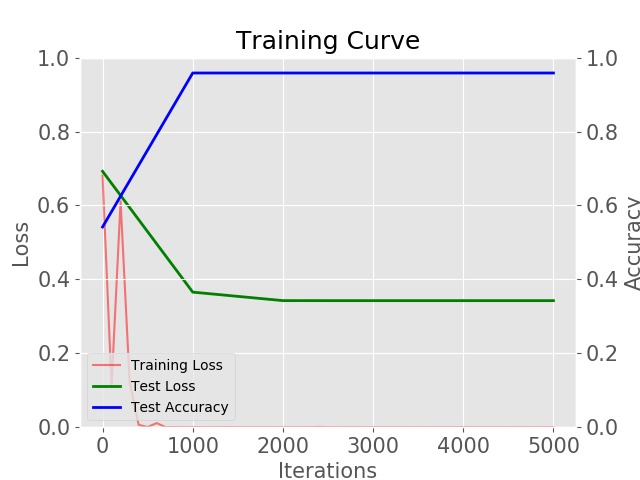
\includegraphics[width=2.5in]{img/curve_vgg16.png}
    \caption{Acurácia e perda de treino e validação da rede VGG16 com transfer learning.}
    \label{fig:acuracia_vgg16_transfer}
  \end{figure}

  \subsection{Resultados sem transfer learning}

  No experimento sem transfer learning, foi utilizada a mesma arquitetura de rede VGG16, porém sem utilizar os pesos pré-treinados. As camadas convolucionais foram inicializadas utilizando o algoritmo xavier \cite{xavier2010}, as últimas camadas totalmente conectadas foram inicializadas utilizando valores de distribuição normal com desvio padrão $0.01$.

  O treino foi realizado com $10000$ iterações, utilizando mini batches de 20 imagens e gradiende descendente estocástico. A taxa de aprendizagem foi inicializada em $0.1$ e diminuída a cada $5000$ iterações, utilizando a equação \ref{eq:learning_rate}. Os parâmetros de momentum e e weight decay não foram alterados, utilizando os mesmos definidos no experimento com transfer learning. Para evitar que os gradientes aumentassem muito, foi utilizada a técnica de gradient clipping para que os gradientes não sejam maior que $1$.

  %iterações e tempo de processamento
  %grafico da acuracia

\section{Discussão}

%dificuldades para definir os parametros corretos de treinamento
%dataset pequeno, precisa de mais dados



\section{Conclusão}



%Use BIB file
\bibliographystyle{abntex2-num}
\bibliography{template}

% that's all folks
\end{document}


